\chapter[Annexes]{Annexes}
\thispagestyle{firstpage}

\minitoc
\newpage

\section{Article 3}\label{article3}
\includepdf[scale=0.85,pages=1-6,pagecommand={\thispagestyle{normalpage}}]{figures/articles/pico-2023.pdf}

\section{Article 1 - Suppl. Data 1}
\textbf{Suppl. Data 1 - Distribution of deltas of node of birth of genes encoding proteins involved in all the pathways, according to the node of birth of each gene}\\
Legend: Deltas are calculated via clade of birth rank for the A gene - clade of birth rank for the B gene for the interaction A $\rightarrow$ B. For example, if gene A was born at the blue clade (clade 1), and the clade of birth of B is 11, the A $\rightarrow$ B delta is -10. Moreover, in this case, it is a backward relationship, because A was born before B.
\par The pathways are in the following order:
PPAR, MAPK, ErbB, Ras, Rap1, Calcium, cGMP-PKG, cAMP, Chemokine, NF-kappa B, HIF-1, FoxO, Sphingolipid, Phospholipase D, p53,  mTOR, PI3K-Akt, AMPK, Wnt, Notch, Hedgehog, TGF-beta, VEGF, Apelin, Hippo, Toll-like receptor, NOD-like receptor, RIG-I-like receptor, C-type lectin receptor, JAK-STAT, IL-17, T cell receptor, B cell receptor, Fc epsilon RI, TNF, Neurotrophin, Insulin, GnRH, Ovarian steroidogenesis, Estrogen, Prolactin, Thyroid hormone, Adipocytokine, Oxytocin, Glucagon, Relaxin, AGE-RAGE.

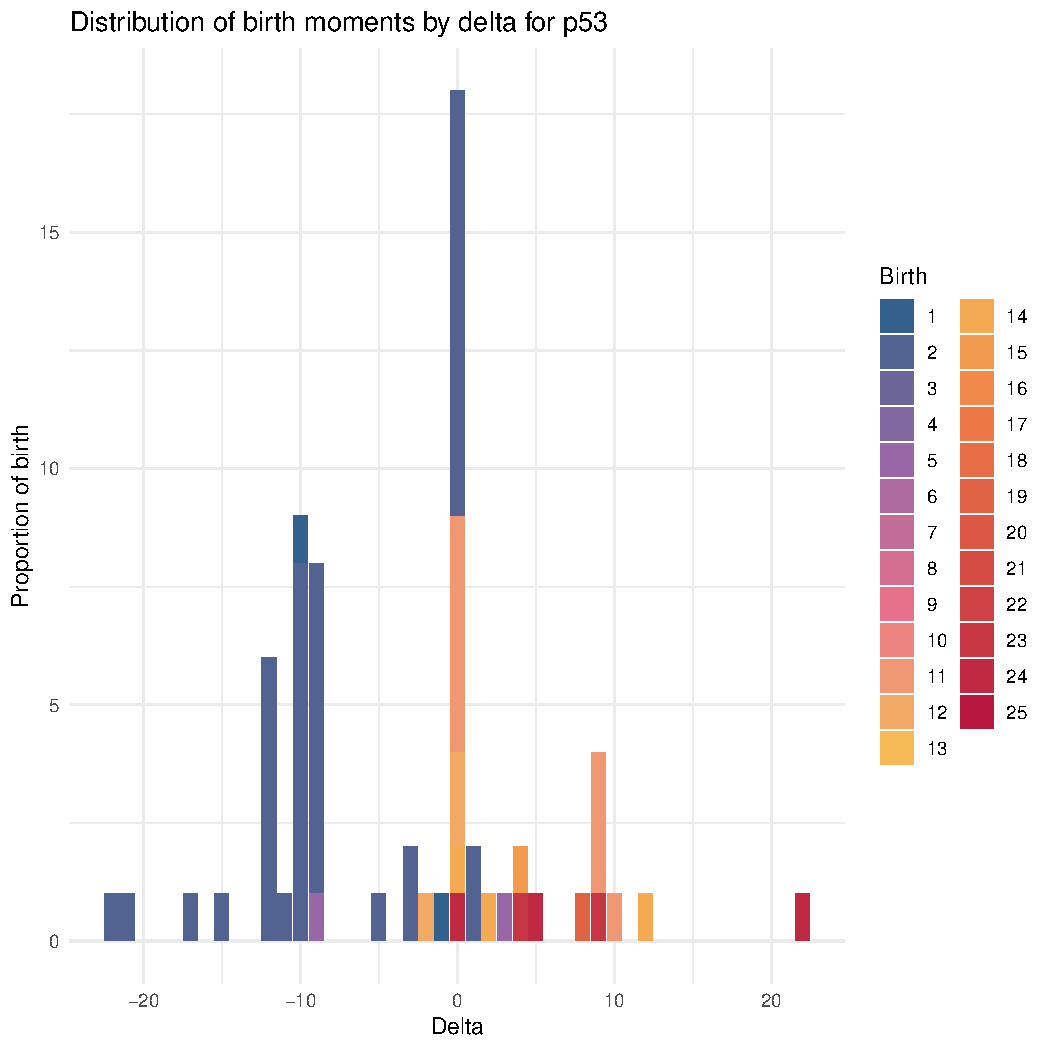
\includepdf[scale=0.85,pages=1-47, nup=1x2, pagecommand={\thispagestyle{normalpage}}]{figures/suppldata/suppldata1.pdf}

\section{Article 1 - Suppl. Data 2}
\textbf{Suppl. Data 2 - Colored KEGG pathways depending on the node of birth of each protein}\\
Legend: Each color represents a clade. The white rectangles correspond to the genes for which we have not been able to determine the node of birth due to lack of information about the gene. The KEGG legend is available here: \href{https://www.genome.jp/kegg/document/help_pathway.html}{https://www.genome.jp/kegg/document/help}
\par The pathways are in the following order:
PPAR, MAPK, ErbB, Ras, Rap1, Calcium, cGMP-PKG, cAMP, Chemokine, NF-kappa B, HIF-1, FoxO, Sphingolipid, Phospholipase D, p53,  mTOR, PI3K-Akt, AMPK, Wnt, Notch, Hedgehog, TGF-beta, VEGF, Apelin, Hippo, Toll-like receptor, NOD-like receptor, RIG-I-like receptor, C-type lectin receptor, JAK-STAT, IL-17, T cell receptor, B cell receptor, Fc epsilon RI, TNF, Neurotrophin, Insulin, GnRH, Ovarian steroidogenesis, Estrogen, Prolactin, Thyroid hormone, Adipocytokine, Oxytocin, Glucagon, Relaxin, AGE-RAGE.

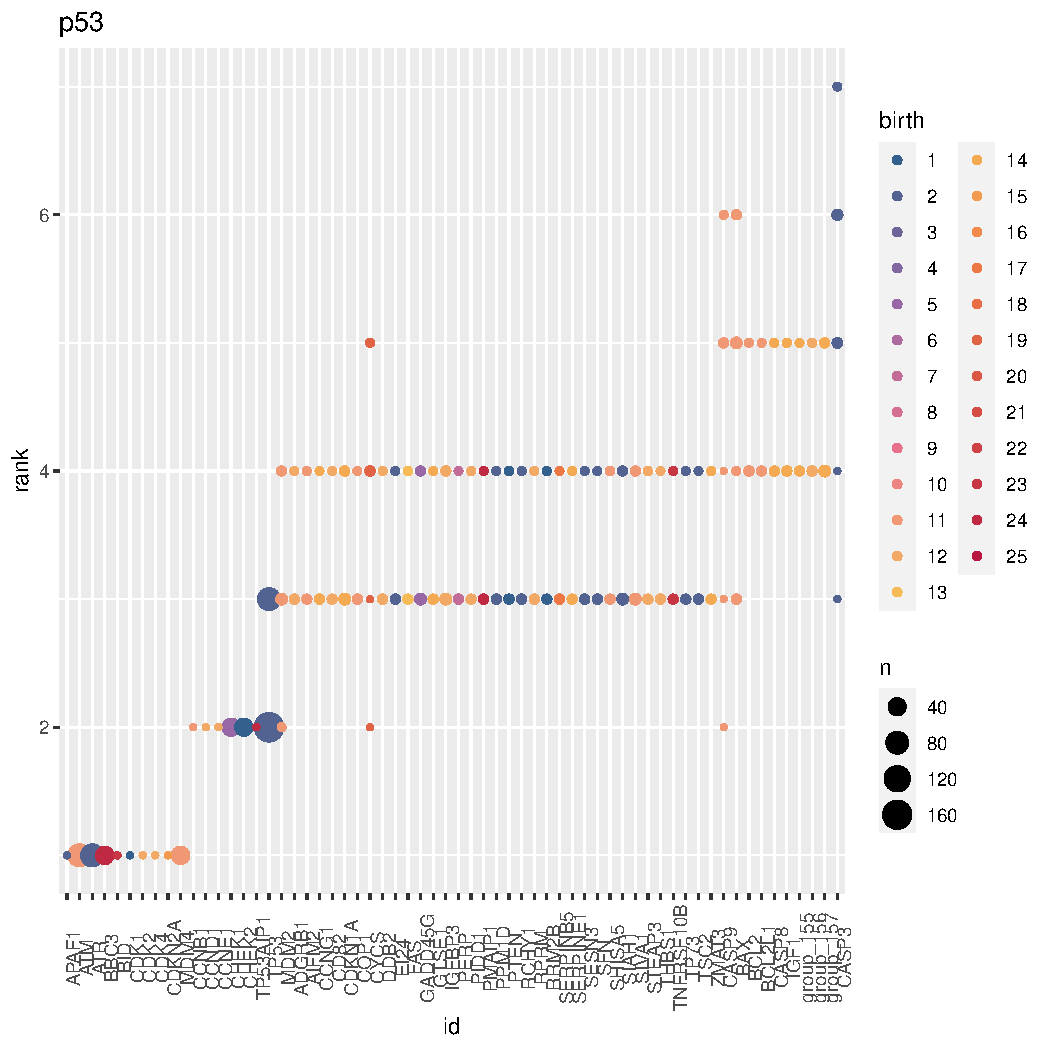
\includepdf[scale=0.85,pages=1-47, nup=1x2, pagecommand={\thispagestyle{normalpage}}]{figures/suppldata/suppldata2.pdf}

\section{Article 1 - Suppl. Data 3}
\textbf{Suppl. Data 3 - Animal tree of life and clades of study}\\
Legend: Tree of life of the 315 species studied here, generated using the information available in Ensembl and Ensembl Metazoa, and with R's ape package \parencite{paradis_ape_2019}. The tree is rooted to reflect the phylogeny of the \textit{Opisthokonta}, and the branches are not to scale. The colors are those used in the figures of the article. Each clade is represented by one or more species in our database.

\includepdf[scale=1, pagecommand={\thispagestyle{normalpage}}]{figures/suppldata/suppldata3.pdf}

